A RandomVariable object is a combination of a DiscreteRandomVariable and a ContinuousRandomVariable objects. The continuous case is the focus since it's more challenging. 

Furthermore the focus at this level is one dimensional functions of random variables. Such functions are built up of components such as addition or multiplication by a constant, exponential powers such as $X^2$ as well as sums, difference, products and quotients of functions of the same random variable. The function that will form a running example in this section is,

\begin{align*}
Z = \ln(X + X^2)
\end{align*}

This is more generally expressed as,

\begin{align*}
Z = h(f(X) * g(X))
\end{align*}

where $*$ represents any binary operator such as $+, -, \times, \text{and } \div$.

\subsection{One Dimensional Functions of a Continuous Random Variable}

The goal of representing a continuous random variable is for the purpose of plotting it's probability density function for the user. We suppose that plotting a probability density function involves providing a partition of the real line. The software must then provide accurate estimates of the probability between each adjacent pair of partition elements. In an abuse of notation we write the partition of the resulting $Z$ random variable to be plotted as,

\begin{align*}
Z \sim (z_1, ..., z_{n+1})
\end{align*}

Then for each $i \in 1..n$ we must compute $Pr(z_i < Z \le z_{i+1})$. If $Z$ were a function of two random variables $X$ and $Y$ then each partition endpoint $z_i$ corresponds to a iso-curve in $(X,Y)$-space. This is still the case, but the iso-curves are isolated points, or possibly intervals in the case of function degeneracy.

The partition elements of the partition of $Z$ are indexed by their left-hand endpoint index. There are $n$ such partition elements. For each the software must locate the pre-image and compute the probability of this subset of the domain of $X$. The advantage of knowing all the range intervals at once and in particular knowing they are non-overlapping.

The running example $Z = \ln(X + X^2)$ is represented by the tree \ref{fig:ln_x_plus_x2}

\begin{figure}
  \centering
  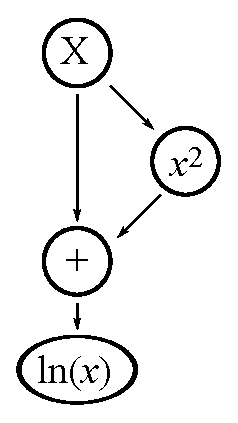
\includegraphics{Images/ln_x_plus_x2.eps}
  \caption[Tree of $Z = ln(X + X^2)$]
          {Tree of $Z = ln(X + X^2)$}
  \label{fig:ln_x_plus_x2}
\end{figure}


The basic algorithm to compute the pre-image of the $Z$ partition (itself a partition) is,

\begin{enumerate}
\item If any function block is of form $x^{-|p|}$ find and mark the pole in the $X$ domain.
\item Pick an initial $x$-value. The median may be the most convenient.
\item Ensure that each function block in the tree satisfies the domain requirements.
\item If domain requirements are not satisfied then find the extents of the domain violation.
\item For the working $x$-value find the extents of the current partition.
\item For each unidentified interval in the $X$ domain, goto step 2.
\end{enumerate}

The algorithm requires much explaining. The first step is the \emph{pole identification} step. There are no poles in the running example. If one of the blocks is of the form $x^{-2}$, for example, then we trim the tree before the reciprocal block and perform a root-finding step.

\subsubsection{Root Finding}

Given a function $f(X)$ we want to find all values $x \in X$ so that $f(x) = 0$. The general state of $X$ is that some or all poles are identified with some bounding interval and some or all domain violation regions are similarly marked with a bounding interval. If the root finding step is taking place in the context of initial pole identification then no regions will yet be indentified as the pre-image of the $Z$ partition since it's not yet specified.

Each unexplored region in $X$ must be explored for a possible. The bounded Halleys Algorithm is detailed below. It requires the computing of the first and second derivatives of $f(X)$ where we suppose,

\begin{align*}
g(X) = f(X)^{-|p|}
\end{align*}

A significant issue is finding the multiple roots, if any. A saving grace is that we work from the inside out. There should be no unidentified poles in $f(X)$. This means that if we chase a tail and we don't have a boundary in front of us we can safely mark the extents as explored. Using Halley's Method (bounded or unbounded) we always explore both directions from the initial $x$.

Another feature we might consider is the identification of polynomial expressions. Polynomial root-finding is a special case. Linear is even more special. 
